% ligo_south_study.tex

We currently plan to have three \ac{LIGO} detectors when Advanced LIGO comes online: one interfermeter at Livingston, L1, and two at Hanford: H1 and H2. H2 is planned to have $4\,$km arms, instead of the $2\,$km length it had in initial LIGO. However, in the past year the possibility opened up for a \ac{LIGO} interfermeter to be built in Australia. In this case, LIGO would still have three interferometers; rather than have two at Hanford, the optics for H2 would be shipped to the Australian site to be set up there.

\section{Advantages of LIGO South}

A number of studies were carried out to evaluate the pros and cons of having a H1L1S1 (S1 for the Austrialian detector) network as opposed to a H1H2L1 network. Most of these studies found that the H1L1S1 network had a number of advantages over the H1H2L1 network. Perhaps the biggest benefit is sources can be better localized if the third detector is in the southern hemisphere. Since the interferometers are not directional antennas, a network is needed to localize a source. Essentially, by measuring the difference in time of arrival between the various detectors in the network, we can triangulate the source (our brains do this to localize sounds, where the detectors are our ears). How well we can localize a source is given by \cite{Fairhurst2009, wiki:ligoSth:localization}:
\begin{equation*}
p(\mathbf{r}|\mathbf{R}) \propto p(\mathbf{r})\exp\left[ -\frac{1}{2}(\mathbf{r} - \mathbf{R})^T \mathbf{M}(\mathbf{r}-\mathbf{R})\right]
\end{equation*}
where $\mathbf{R}$ is the actual location, $\mathbf{r}$ is the reconstructed location, $p(\mathbf{r})$ is the prior distribution on $\mathbf{r}$, and $\mathbf{M}$ is given by:
\begin{equation*}
\mathbf{M} = \left[\sum \sigma_i^{-2}\right]^{-1} \sum_{i<j} \frac{\mathbf{D}_{ij}\mathbf{D}^T_{ij}}{\sigma^2_i \sigma^2_j}
\end{equation*}
Here, $\sigma_i$ is the timing accuracy in the $i\th$ detector and $\mathbf{D}_{ij}$ is the distance between the $i\th$ and $j\th$ detectors. Thus, the larger the distance between any two detectors, the more strongly peaked the probability distribution will be around the actual location.

It was found \cite{wiki:ligoSth:localization} that in the H1L1S1 network, an optimally located\footnote{Optimally located means the source is overhead the plane of the detector. The worst localization occurs when the source is in the plane of the detectors. The numbers presented are therefore best-case scenarios.} source at \ac{SNR} 7 could be localized to an area of $8.5$ square degrees with $90\%$ probability. In the H1H2L1 network the best localization was $12.5$ square degrees. If Virgo is added to the network, then with H1L1S1V1 the localization can be as small as $2.8$ square degrees with $90\%$ probability, whereas it is $10.0$ square degrees with H1H2L1V1.

Another advantage of an Australian detector, as opposed to two at Hanford, is all the detectors can be slid relative to each other. Recall that in \ac{S5} we could not analyze H1H2 time because of the correlated noise. Further, if there was some environmental factor that caused one of the Hanford detectors to lose lock, it would most likely also cause the other Hanford detector to lose lock. This hurt our duty cycle. If we instead have three non-co-located detectors, then we increase the probability that at least two detectors will be up at any given time, thereby increasing our total observation time.

\section{Can We Detect at SNR 8 with Two Detectors?}

There were a number of clear advantages to moving the second Hanford detector to Australia. However, one concern about doing this was the effect it would have on the Advanced LIGO projected chronology. If the optics for the second Hanford detector were packed up and shipped to Australia, it would likely take an additional two or more years to get the detector operational. This means that for the first few years of Advanced \ac{LIGO}, we would only have two detectors.\footnote{There is also the Virgo detector, but as Virgo is maintained and funded by a different collaboration, they may not have the same schedule as \ac{LIGO}. Thus, in this study we wanted to focus on what could be done with strictly the \ac{LIGO} detectors.} Our projected detection rates are based on being able to detect binaries at an \ac{SNR} of $8$. The concern was, if we only have two detectors, can we confidently detect a \ac{GW} at \ac{SNR} $8$? If we could not, then we would not build \ac{LIGO} South.

To answer this question we looked at the rates of H1L1 coincidences in \ac{S5}. We used \ac{S5} as opposed to \ac{S6} because \ac{S6} was still going on when we addressed this question. All of the months from the 12--18 month analysis were used, along with four months from the \ac{S5}-LV analysis. All H1L1 coincidences were used in double-, triple- and (in the case of the LV months) quadrupule- coincident times. For H1H2L1, H1L1V1, and H1H2L1V1 coincidences, the H1L1 part of the coincidence was used to re-calculate the combined new \ac{SNR} of the trigger.

Figure \ref{fig:ligo_south-cat3_newsnr} shows the result of the analysis for the low chirp-mass bin ($\mchirp < 3.48$). Plotted is the cumulative rate of zero-lag (``Foreground") and slide (``Background") triggers as a function of combined new \ac{SNR}. The slide triggers were generated from the standard 100-slide \ihope analysis. The y-axis was generated in the same manner as in the cumulative-rate plots in Figures \ref{fig:} of Chapter \ref{ch:s6_results}. Indeed, these plots were a predecessor to the rate plots shown in Chapter \ref{ch:s6_results}. The dashed-red line shows what the combined new \ac{SNR} would be for signal with \ac{SNR} $8$ in each detector ($= 11.3$). Also plotted, as a yellow star, is the combined new \ac{SNR} of a blind \ac{CBC} injection that was made during \ac{S5}. (This injection, which was in the \ac{S5}-LV analysis, was missed because it occurred when an earthquake was passing Livingston, resulting in L1 being CAT3 vetoed during the time. For more details on this blind injection, see \cite{S5LowMassLV}.)

It is evident from the plot that an event with a new \ac{SNR} of $8$ in each detector would stick out above the background. In this case, we would place an upper-limit on the \ac{FAR} as being $< 1$ in $50$ years. We can arrive at the same conclusion from looking at Figure \ref{fig:?} of Chapter \ref{ch:s6_results}. (Recall that these plots were also created using only H1L1 triggers.) There we can use the extrapolation to estimate what the \ac{FAR} would be for an signal with combined new \ac{SNR} of $11.3$. In the low chirp-mass bin we would have a \ac{FAR} $\approx 1$ in $10^4$ years. 

\subsection{Caveats}

There are a few caveats to this analysis. First, note that we have shown results after CAT3 vetoes have been applied. Figure \ref{fig:ligo_south-newsnr_cat2} shows the same plot as in Figure \ref{fig:ligo_south-money_plot} after CAT2 vetoes have been applied. In this plot we can see that an event at \ac{SNR} $8$ in each detector \emph{would not} stick above the background; it would only have a \ac{FAR} of $\sim1$ in $3$ years. This highlights the importance of \ac{DQ} investigations. Without good data-quality, we cannot detect at \ac{SNR} $8$ using two detectors.

Second, note that we have plotted results as a function of combined \emph{new} \ac{SNR}. Figure \ref{fig:ligo_south-snr_cat3} shows the results after CAT3 as a function of combined \ac{SNR}. The large tail due to non-Gaussian transients has buried the \ac{SNR} 8/8 line in background; such an event would have a \ac{FAR} of $\sim1$ in $30$ years if combined \ac{SNR} was our ranking statistic. Clearly, without new \ac{SNR} we could not detect at \ac{SNR} $8$ (or $40$, for that matter). However, when talking about real events, we have interchanged new \ac{SNR} and \ac{SNR}: we quote rates based on a \emph{\ac{SNR}} of $8$ in each detector, yet we have placed the red-dashed line at a \emph{new \ac{SNR}} of $8$ in each detector. The reason we can do this is new \ac{SNR} reduces to \ac{SNR} for (well-modelled) \acp{GW}. Figure \ref{fig:ligo_south-newsnr_v_snr} shows a plot of combined new \ac{SNR} versus combined \ac{SNR} for (non-spinning) injections. The vertical dashed line shows the combined $\rho = 11.3$ point. At this point, we can see that most of the injections have a combined new \ac{SNR} $> 11$. Note that some of the lower points are due to glitches being mistakenly mapped to injections; c.f. Figure \ref{fig:ligo_south-inj_mchirp_accuracy}. Thus to detect with two detectors at the quoted rates, we need new \ac{SNR}, which in-turn requires that we have templates the well-match the \ac{GW} signal.

Finally, note that we have so far only shown plots for the low chirp-mass bin. The background does not fall off as sharply in the higher chirp-mass bins. This can be seen by comparing Figure \ref{fig:?} to Figure \ref{fig:?}: the medium chirp-mass bin has a higher tail, leading to larger \acp{FAR} at the same new \ac{SNR}. However, as can be seen in the extended background with the blind injection removed (the gray crosses) in Figure \ref{fig:?}, we would still get a \ac{FAR} of $~1$ in $3500$ years in the medium chirp-mass bin at a combined new \ac{SNR} $11.3$. Though higher than the low chirp-mass bin, this \ac{FAR} is still low enough to claim evidence for a detection. Further, we are most concerned with the low chirp-mass bin, as this contains \ac{BNS} systems. Out of \ac{BNS}, \ac{BBH} and \ac{NSBH} systems, the rate of \ac{BNS} coalescence in the universe is the best constrained, as it is based on actual astrophysical observations of \ac{BNS} systems. We are therefore most confident in quoted expected rates of detection for \ac{BNS} coalescence, and so it is for these systems that we wish to ensure that we can detect at \ac{SNR} 8.

\section{Conclusions}

This study showed that building \ac{LIGO} South would not hamper our abilities to detect \ac{GW} at the quoted rates in the near term. Thus the decision of whether or not to build \ac{LIGO} South can be based solely on the availability of funds. Regardless of whether or not \ac{LIGO} South is built, this study proved useful, as it gave us confidence that we can detect \acp{GW} at expected rates in Advanced LIGO. Admittedly, we cannot be certain that the character of the noise will be the same in Advanced LIGO. However, by comparing the \ac{S5} cumulative rate plot in this chapter to the corresponding \ac{S6} plots in Chapter \ref{ch:s6_results}, we see that we obtained largely the same (better, even) background distribution in \ac{S6}, despite a number of hardware differences between the runs. Thus, by making using of new \ac{SNR}, and with equally intensive \ac{DQ} studies in Advanced \ac{LIGO}, we can expect to detect at a \ac{SNR} of $8$ in each detector.

\begin{figure}[p]
\center
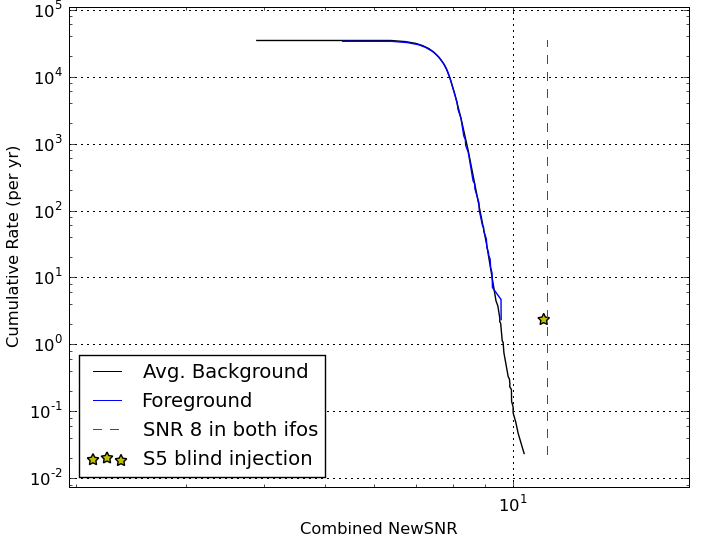
\includegraphics[width=6in]{figures/ligo_south/Cat3-newsnr-low_mass.png}
\label{fig:ligo_south-cat3_newsnr}
\caption{Cumulative rate of H1L1 zero-lag (``Foreground") and slide (``Background") coincidences in \ac{S5} after CAT3 (cumulative) vetoes have been applied. Only triggers in the low chirp-mass bin ($\mchirp < 3.48\,\Msun$) are shown. Data used is from all of the \ac{S5} 12-18 months, plus four months from the \ac{S5}-LV analysis. The black line indicates the background; the blue line indicates the foreground. As with the cumulative rate plots in Chapter \ref{ch:s6_results}, the foreground rates are computed by dividing the cumulative count of foreground triggers by the total zero-lag live time ($T_{\mathrm{f}}$). The background rates are computed by dividing the cumulative count of background triggers by total slide live time ($T_{\mathrm{b}}$), which is equivalent to divding by the effective number of slides ($= T_{b}/T_{f}$), then dividing by the zero-lag live time. Hence the black line is labelled as the ``Average Background." The red-dashed line indicates the combined new \ac{SNR} for an event with single-\ac{IFO} new \ac{SNR} of $8$ in each detector. The yellow star shows the combined new \ac{SNR} of a blind injection that was made during the \ac{S5}-LV analysis.}
\end{figure}

\begin{figure}[p]
\center
\subfigure[After CAT2 vetoes applied.]{\label{fig:ligo_south-newsnr_cat2}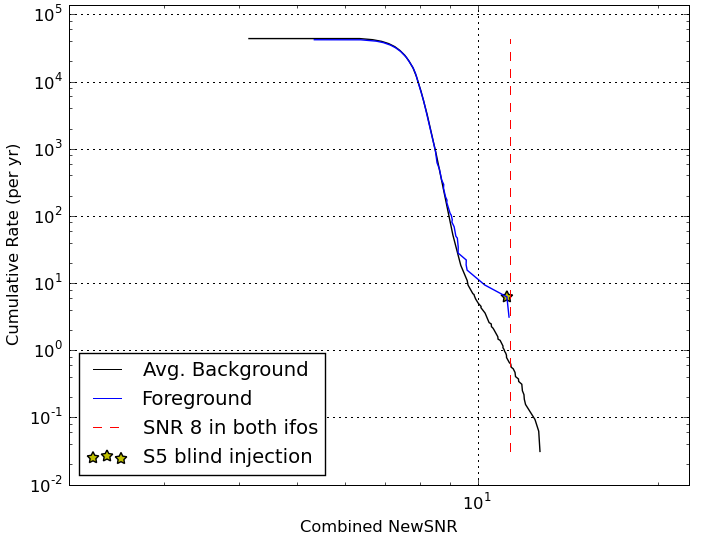
\includegraphics[height=3.5in]{figures/ligo_south/Cat2-newsnr-low_mass.png}}
\subfigure[Cumulative rate vs. combined \ac{SNR}, after CAT3 vetoes applied.]{\label{fig:ligo_south-snr_cat3}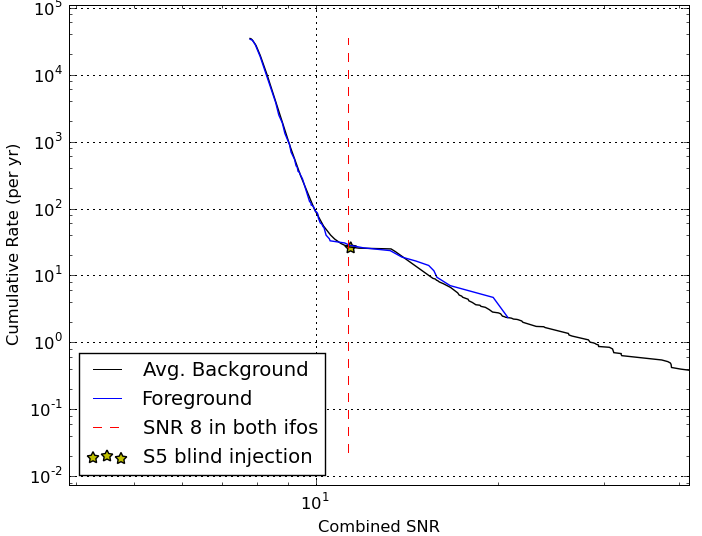
\includegraphics[height=3.5in]{figures/ligo_south/Cat3-snr-low_mass.png}}
\label{fig:ligo_south-cat2_and_snr}
\caption{Cumulative rate plot for the same period of time shown in Figure \ref{fig:ligo_south-cat3_newsnr}, after CAT2 vetoes have been applied (top) and as a function of combined \ac{SNR} (bottom). In the bottom plot, CAT3 vetoes have been applied.}
\end{figure}

\begin{figure}[p]
\center
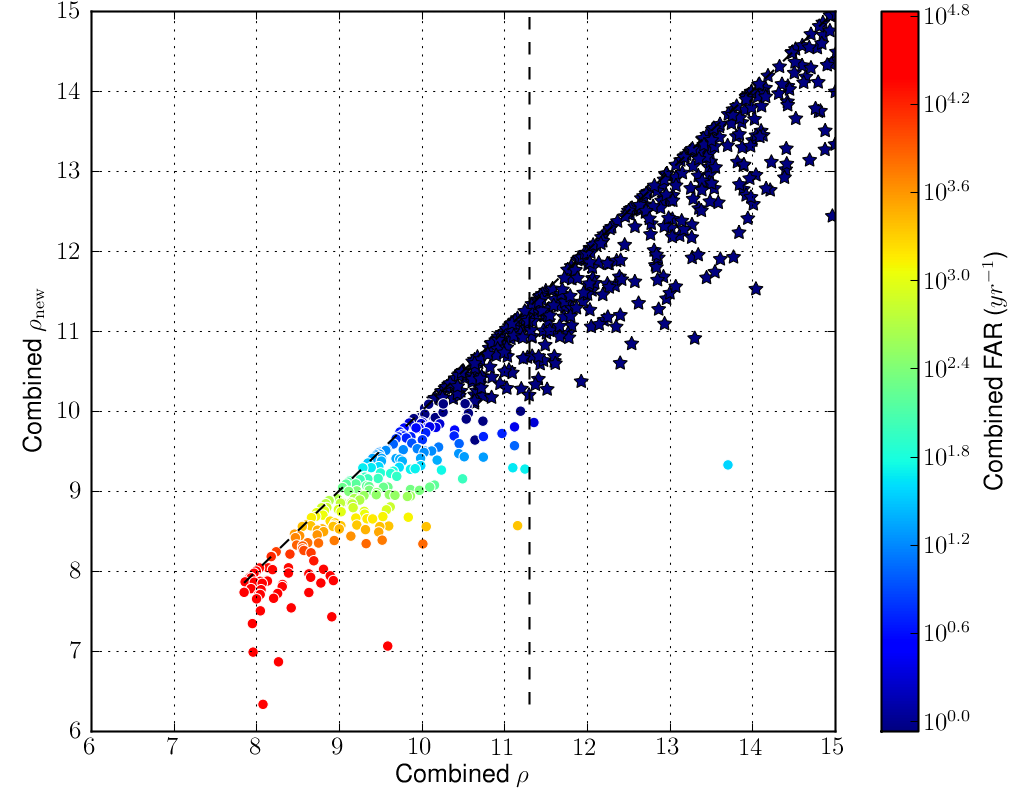
\includegraphics[width=6in]{figures/ligo_south/H1L1-ligolw_cbc_plotfm_Non-Spinning_mathcalM_mathrminj_0_3_F1_BNSLININJ+BNSLOGINJ+NSBHLININJ+NSBHLOGINJ+BBHLININJ+BBHLOGINJ_PLOTTED-961545543-3628944.png}
\label{fig:ligo_south-newsnr_v_snr}
\caption{Combined new \ac{SNR} versus combined \ac{SNR} for non-spinning injections. All injections were found as H1L1 coincidences. Results taken from $6$ weeks of S6D data. The diagonal black-dashed line indicates $y=x$; the vertical dashed line shows the point where combined \ac{SNR} $= 11.3$. This plot was created by \texttt{ligolw\_cbc\_plotfm}. As with all PlotFM plots, the blue stars indicate injections found with $0$ \ac{FAR} in their analysis period and colored circles indicate injections with non-zero \ac{FAR}.}
\end{figure}

\begin{figure}[p]
\center
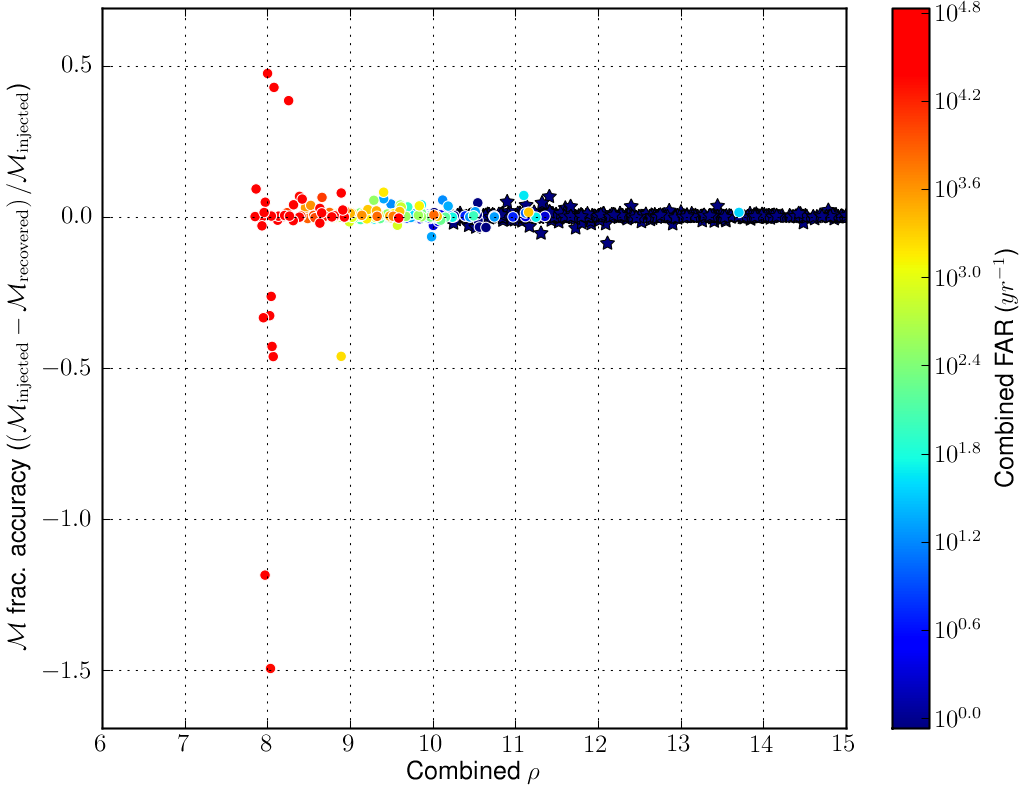
\includegraphics[width=6in]{figures/ligo_south/H1L1-ligolw_cbc_plotfm_Non-Spinning_frac_accuracy_mathcalM_mathrminjected_0_3_F3_BNSLININJ+BNSLOGINJ+NSBHLININJ+NSBHLOGINJ+BBHLININJ+BBHLOGINJ_PLOTTED-961545543-3628944.png}
\label{fig:ligo_south-inj_mchirp_accuracy}
\caption{Recovered chirp mass fractional accuracy of the injections shown in Figure \ref{fig:ligo_south-newsnr_v_snr} as a function of combined \ac{SNR}. Triggers close to zero were most likely caused by injections. Triggers further from the zero line are most likely glitches that happened to be within $\pm 1\,$s of the injection.}
\end{figure}
